%%%%%%%%%%%%%%%%%%%%%%%%%%%%%%%%%%%%%%%%%%%%%%%%%%%%%%%%%%%%%%%%%%% 
%                                                                 %
%                            CHAPTER THREE                        %
%                                                                 %
%%%%%%%%%%%%%%%%%%%%%%%%%%%%%%%%%%%%%%%%%%%%%%%%%%%%%%%%%%%%%%%%%%% 



\chapter{Evaluating for User Interaction in Spatially Augmented Reality Systems}


In well designed user interfaces, it is imperative to run user studies to verify the user experience meets design expectations.  I have taken lead on running three studies on the tabletop system.  The first study involved collecting designs made my students on the tabletop.  Because designs need to be closed off and made into a mesh there is often a certain amount of ambiguity in creating a closed space.  The second user study tested if architects agreed with how the remesher’s algorithm (designed by Barb Cutler) interpretted the closed space.  Once we were convinced this was the case (involving a pilot study, some modifications and a continuation of the study), we ran another study which tested how well users were able to model using the tool and how well the system communicated daylighting information to the modelers.  Finally, we ran a user study which used the same system in a non-daylighting application, an  army battle simulation game.  From this study we gained several insights into augmented tabletop games and how they compare to non-augmented games.
%\begin{figure}[p]
%\resizebox{0.74in}{0.725in}{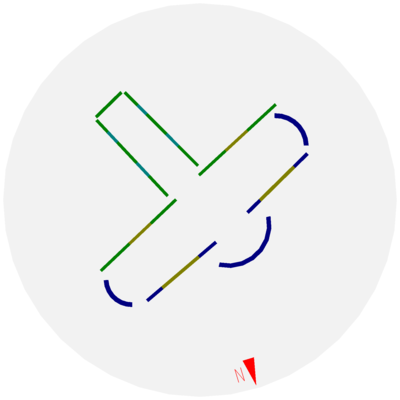
\includegraphics{images/011_detected_02605_small}}
%\resizebox{0.74in}{0.725in}{
\includegraphics{images/011_annotated_02605}}
%\resizebox{0.74in}{0.725in}{
\includegraphics{images/011_02605_floorplan_small}}
%
%\resizebox{0.74in}{0.74in}{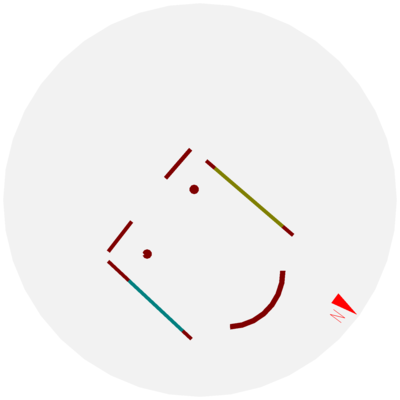
\includegraphics{../uist2012/images/appendix/012_detected_03882_small}}
%\resizebox{0.74in}{0.74in}{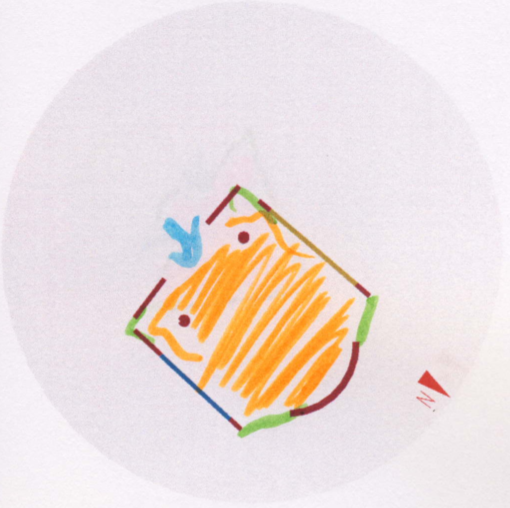
\includegraphics{../uist2012/images/appendix/012_annotated_03882}}
%\resizebox{0.74in}{0.74in}{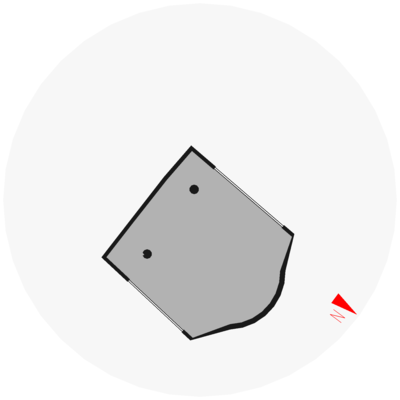
\includegraphics{../uist2012/images/appendix/012_remeshed_03882_small}}
%
%
%\resizebox{0.74in}{0.725in}{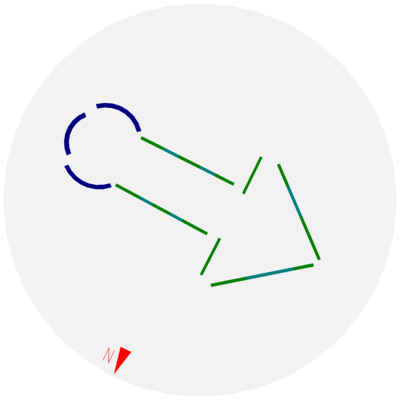
\includegraphics{images/012_detected_05563_small}}
%\resizebox{0.74in}{0.725in}{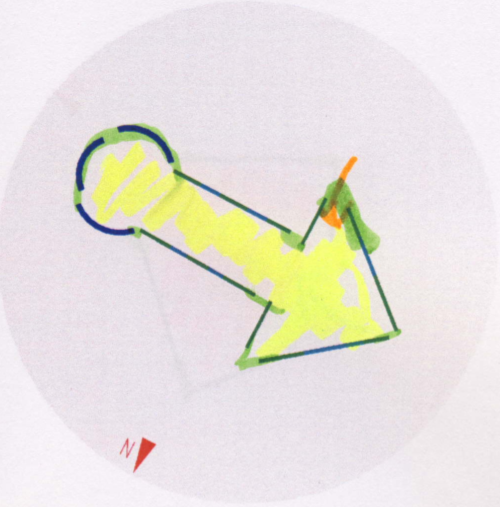
\includegraphics{images/012_annotated_05563}}
%\resizebox{0.74in}{0.725in}{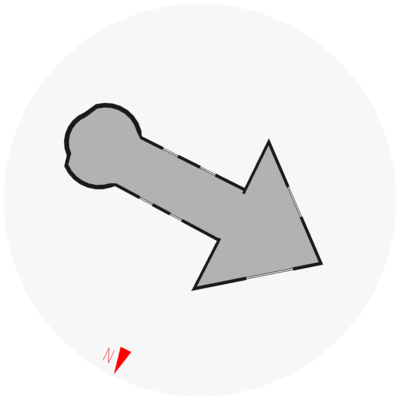
\includegraphics{images/012_remeshed_05563_small}}
%\\
%\resizebox{0.74in}{0.725in}{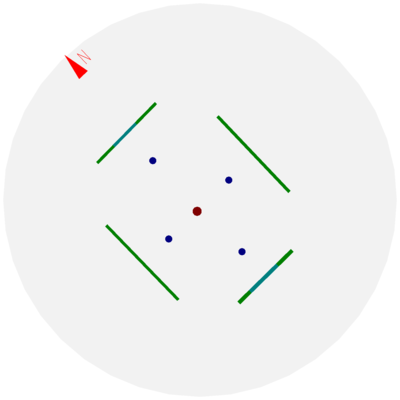
\includegraphics{images/024_detected_02694_small}}
%\resizebox{0.74in}{0.725in}{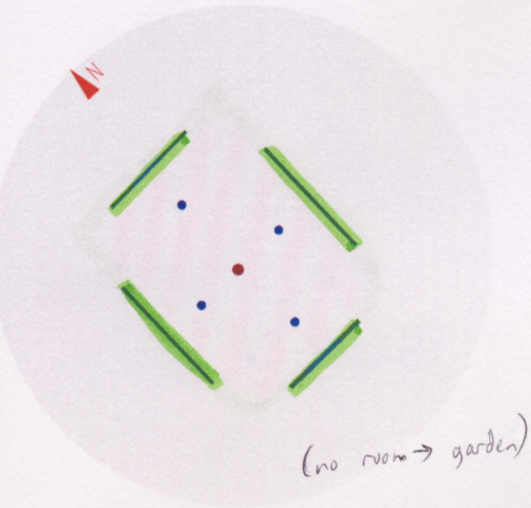
\includegraphics{images/024_annotated_02694}}
%\resizebox{0.74in}{0.725in}{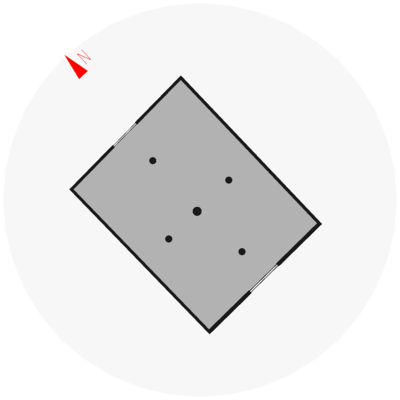
\includegraphics{images/024_remeshed_02694_small}}
%resizebox{0.74in}{0.725in}{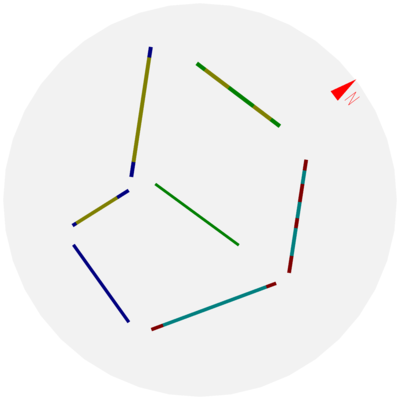
\includegraphics{images/097_detected_11365_small}}
%\resizebox{0.74in}{0.725in}{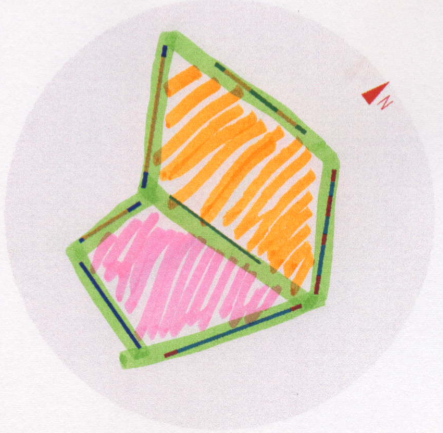
\includegraphics{images/097_annotated_11365}}
%\resizebox{0.74in}{0.725in}{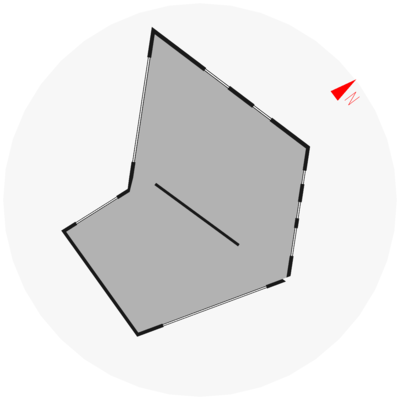
\includegraphics{images/097_remeshed_11365_small}}



